
\def\theTopic{Glossary }
\def\dayNum{  }

\section{Glossary}

\begin{center}
 {\large\bf  Unit 1 Definitions:}
\end{center}
\begin{description}
\item [Cases:] subjects or units that information is collected on (Descriptive Statistics Video)
\item [Variable:] the characteristics that are recorded for each case
  (Reading 1 and Activity 1; Descriptive Stats Video)
\item [Categorical Variables:] tells us some attribute of the case
  which is not numeric; data falls into one of two or more categories;
  summarized with tables and proportions (Reading 1 and Activity 1;
  Descriptive Stats Video)
\item [Quantitative Variables:] numbers that can be average together;
  summarized with the mean or median and spread (Reading 1 and
  Activity 1; Descriptive Stats Video)
\item [Measures of Center:]  (Reading 1)
  \begin{list}{}{}
  \item [Mean:] the average of the sample; found for symmetric
    distributions
  \item [Median:] the center data point; found for skewed
    distributions or for distributions with outliers; the measure of
    center is resistant to outliers 
  \end{list}

\item [Measure of Spread:] (Reading 1)
  \begin{list}{}{}
  \item [Standard deviation:] measures the spread of each data point
    from the mean
  \item [Interquartile Range (IQR):] Q3-Q1 – measures the spread of
    the data from the median 
  \end{list}

\item[Population:] all the cases (units) of interest (Reading 2) 
\item [Sample:] a subset of the population that gets measured or
  observed in our study; sample size is denoted by n (Reading 2)
\item [Convenience Sample:] a sample that is made up of units which
  are easy to measure; does not represent the population (Reading 2)
\item [Non-response bias:] occurs when people do not respond to a
  survey (Reading 2)
\item [Simple Random Sample:] a sample method in which every sample of
  size n has the same chance of being selected (Reading 2) 
\item [Stratified Sample:] a sample method in which the population is
  divided into strata before simple random sampling is employed
  (Reading 2)
\item [Statistical Inference:] making a statement about a population
  parameter based on a sample statistic (Reading 2)
\item [Parameter:] describes the characteristics of the population (Reading 2)
\item [Statistic:] describes the characteristic of the sample and is
  computed from the sample; also called the observed result or the
  point estimate (Reading 2)
\item [Parameter of interest for single categorical variable:]  the
  true proportion of (context)\\
  {\bf Example:} $p$ – the true proportion of MSU students who drive
  FORD vehicles
\item [Unbiased:] a sample that is representative of the population or
  a statistic with sampling distribution centered at the parameter of interest. 
\item [Precision:]  the larger the sample size the less variability
  within the sample (more precise)
\item [Strength of Evidence (p-value):] the probability of seeing the
  observed result or more extreme if the null hypothesis is true
  (Activity 4)\\
   {\bf Interpretation of a p-value:} There is a (\_\_p-value)\_\_\% chance
   of the observed result of \_(statistic)\_ or more extreme occurring
   if the null hypothesis is true (in context) (Activity 4)
 \item [Hypothesis Test:] test to show evidence based on the sample
   statistic against the null hypothesis (Activity 4) \\
    {\bf Null hypothesis for a single proportion:} the true proportion
    of  (context)  is equal to  (null hypothesized value)
    $$ H_0: p = p_0$$
    {\bf Null Distribution:} distribution created based on the
    assumption that the null hypothesis is true; centered at the null
    value (Activity 4)
  \item [Confidence Interval:] provides an estimate of the true
    parameter (Activity 6)
  \item [Bootstrapping:] resample with replacement from the original
    statistic (Activity 6) \\
    {\bf Bootstrap Distribution:} distribution created by resampling
    with replacement from the original statistic; centered at the
    original statistic (Activity 6)
  \item [Percentile Method:] method to create confidence intervals
    where the middle \_(level of confidence)\_\_\% is included in the
    interval and the remaining \% is excluded (Activity 6)
  \item [2SE Method:]  point estimate plus or minus 2 times the SE of
    the statistic where 2 is the multiplier for the 95\% confidence
    interval; only used for categorical data
  \item [Margin of Error:] multiplier times the SE of the statistic;
    the amount we add to and subtract from our estimate.
  \item [Confidence Interval formula for 2SE Method for a single
    proportion:] $$ \phat \pm 2\times SE(\phat)$$
  \item [Plausible Value:]  A possible value for the parameter which
    is close enough to the estimate to be included 
    within the confidence interval.
  \item [Interpretation of a Confidence Interval (one categorical):]
    We are \_(level of confidence)\_\_\% confident the true proportion
    of \_\_(context)\_\_ is between \_\_(interval)\_\_. (Activity 7)
  \item [Meaning of Confidence (one categorical):] Approximately
    \_(level of confidence)\_\% of random samples will create a
    \_(level of confidence)\_\% confidence interval that contains the
    true \_\_(parameter of interest in context)\_\_. (Activity 7)
  \end{description}\vspace{1cm}
  
  \begin{center}
    {\large\bf Unit 2}
  \end{center}
  \begin{description}
  \item[Experiment:] studies in which treatments are assigned to the
  cases (units) of the study (Reading 8)
\item [Randomized Experiments:] those in which treatments are randomly
  assigned to cases (units) (Reading 8)
\item [Observational Study:] studies in which no variables are set,
  but each is simply observed or measured on the cases (units)
  (Reading 8)
\item [Four Principles of Experimental Design:] (Reading 8)
  \begin{itemize}
  \item Control
  \item Randomize
  \item Replication
  \item Blocking
  \end{itemize}

\item [Explanatory Variable:] any factor that can influence the
  response variable.  In an experiment this is the variable in the
  study that the researcher can manipulate and vary (Activity 10 and
  Experiments and Observational Studies Video)
\item [Response Variable:] The outcome variable we observe (our data)
  (Activity 10 and ``Experiments and Observational Studies Video'')
\item [Random Assignment:] when cases are randomly assigned to the
  treatment groups (Activity 10)
\item [Causal Inference:] when the cases are randomly assigned to the
  treatment we can say that the explanatory variable caused the change
  in the response variable (Scope of Inference Video)
\item [Lurking Variable:] a variable not measured in the study that
  may affect the response variable; random assignment of cases to
  treatment evens out the lurking variable between groups and
  eliminates the effects of the lurking variable on the response
  (Activity 10)
\item [Scope of Inference:] the extent to which study results apply to
  other situations. \\
  \begin{tabular}{|l|l|l|}
    & \multicolumn{2}{|c|}{Randomly Assigned?} \\ 
Randomly Selected?& Yes& No\\ \hline
 Yes              & Causal Inference to Population & Association to
 the Population\\ \hline
No &    Causal Inference to Sample & Association to
 the Sample\\ \hline
\end{tabular}
\item [Sampling Distribution:] a description of all possible outcomes
  and the probabilities of obtaining each outcome (Reading 9)
\item [Two Categorical Variables:] Activity 12 and 13\\

  \item [Parameter of interest for difference in proportions:] the
    difference in true proportions of \_\_(context)\_\_
  \item [Null hypothesis for difference in proportions:] there is no
    difference in the true proportion of  \_\_(context group 1)\_\_  and the
    true proportion of   \_\_(context group 2)\_\_ $$ H_0: p_1 = p_2$$
  \item [Confidence Interval formula for 2SE Method for a difference
    in proportions:] $$\phat_1 - \phat_2 \pm 2 \times SE(\phat_1 - phat_2)$$

  \item [Interpretation of a Confidence Interval (two categorical variables):]
  We are \_\_(level of confidence)\_\_\%  confident the true
  proportion of \_\_(context group 1)\_\_ is \_\_(lower CI value )  to
  \_\_(upper CI value)\_\_  \_\_(lower/higher)\_\_ than the true
  proportion of \_\_(context group 2)\_\_.
  \item [Meaning of Confidence (two categorical variables):]
       Approximately \_\_(level of confidence)\_\_\% of random samples
       will create a \_\_(level of confidence)\_\_\% confidence
       interval that contains the difference in true proportion of
       \_\_(context group 1)\_\_ minus the true proportion of \_\_(context
       group 2)\_\_.
     \item [One Categorical and One Quantitative Variable:] Activity
       14
     \item [Parameter of interest for difference in means:] the
       difference in true means (in context)
     \item [Null hypothesis for difference in means:] there is no
       difference in the true mean  \_\_(context group 1)\_\_  and the true
       mean of   \_\_(context group 2)\_\_.
                   $$H_0:\  \mu_1 = \mu_2$$
     \item [Confidence Interval formula for $t^* \times SE$ Method for
       a difference in means:] $$ \xbar_1 -\xbar_2 \pm t^* \times
       SE(\xbar_1 - \xbar_2) $$ 
     \item [Interpretation of a Confidence Interval (one categorical
       and one quantitative variable):] 
       We are \_(level of confidence)\_\%  confident the true mean of
       \_\_(context group 1)\_\_ is \_\_(lower CI value to upper CI
       value)\_\_   \_\_(lower/higher)\_\_ than the true mean
       \_\_(context group 2)\_\_. 
     \item [Meaning of Confidence (one categorical and one
       quantitative variable):] 
       Approximately \_\_(level of confidence)\_\_\% of random samples
       will create a \_(level of confidence)\_\% confidence interval
       that  contains the difference of true mean \_\_(context group
       1)\_\_ minus true mean  \_\_(context group 2)\_\_.
     \item [Single Quantitative Variable:] Activity 11 and 15
       Parameter of interest for single quantitative variable: the
       true mean (context)
     \item [Null hypothesis for single mean:] the true mean  (context)
       is equal to  (null hypothesized value) $ H_0: \mu = \mu_0$
     \item [Confidence Interval formula for $t^*\times SE$ Method for
       a single mean:]$$ \xbar \pm t^* \times SE(\xbar) $$ 

     \item [Interpretation of a Confidence Interval (single quantitative):]
       We are \_\_(level of confidence)\_\_\%  confident the true mean
       \_\_(context)\_\_  is between \_\_(lower endpoint and upper
       endpoint of interval)\_\_.
     \item [Meaning of Confidence (single quantitative):]
       Approximately \_\_(level of confidence)\_\_\% of random samples
       will create a \_\_(level of confidence)\_\_\% confidence
       interval that contains the true mean \_\_(context)\_\_.
     \item [Statistical Significance:] statistical test results that
       provide a p-value less than a cutoff level $\alpha$ are considered
       statistically significant at the $\alpha$ level. (Reading 11) 
     \item [Type I Error:]  probability of rejecting a true null
       hypothesis (Activity 16)
       \begin{itemize}
       \item Reject $H_0$  when in fact $H_0$ is true.
       \end{itemize}
     \item [Type II Error:]  probability of failing to reject a false
       null hypothesis (Activity 16) 
       \begin{itemize}
       \item Fail to reject $H_0$  when in fact $H_0$ is false.
       \end{itemize}
     \item [Power:] probability of rejecting a false null hypothesis
       (Activity 16) 
       \begin{itemize}
       \item How often will we reject $H_0$ when in fact $H_a$ is
         true? (Depends of a particular alternative.)
       \end{itemize}
     \item [Correlation:] measures the strength and direction of the
       linear relationship between two quantitative variables; the
       closer correlation is to $\pm 1$ the stronger the linear
       relationship (Activity 17)
       \begin{itemize}
       \item Notation: $\rho$ for true correlation, $r$ for its estimate.
       \end{itemize}
     \item [Least Squares line:] an estimate of the true relationship
       between predictor $x$ and response $y$.
         $$ \widehat{y} = \widehat{\beta}_0 + \widehat{\beta}_1 x$$
     \item [Slope:] For every 1 increase in the
       predictor ($x$),  the  response $y$
       \_\_(increases/decreases)\_\_   by the slope. State
       $x$ and $y$ in context. (Activity 17)
       \begin{itemize}
       \item Notation: $\beta_1$ for true slope, $\widehat{\beta}_1$
         for its estimate. 
       \end{itemize}
     \item [$y$ intercept:]  The predicted $y$ value
       when our $x$ variable is  .$0$      (Activity 17).
       \begin{itemize}
       \item Notation: $\beta_0$ for true intercept, $\widehat{\beta}_0$
         for its estimate. 
       \end{itemize}
     \item [Residual:]   the difference from the observed y value to
       the predicted y value (Activity 17) 
          $$e = y - \widehat{y} = y - (  \widehat{\beta}_0 +
          \widehat{\beta}_1 x)$$
        \item [Two Quantitative Variables] (Activity 18)\\
          {\bf Null hypothesis for slope:} there is no true linear
            relationship between  (x variable)  and  (y variable) ;
            $H_0:\ \beta_1 = 0$  \\
          {\bf Null hypothesis for correlation:} there is no true
            linear relationship between  (x variable)  and  (y
            variable) ; $H_0:\  \rho = 0$  
        \end{description}
\newpage
        
\begin{center}
  {\large\bf Unit 3}
\end{center}

\begin{description}
\item [Normal Distribution:] theoretical distribution; symmetric,
  bell-shaped,  with  known mean, $\mu$ and standard deviation,
  $\sigma$ (Activity 21)  
  \begin{itemize}
  \item to standardize a random variable, $X$, when $\mu$ and $\sigma$
    are known use $Z = \frac{X-\mu}{\sigma}$.
  \item To find a percentile, solve for $X$:  $ X = Z\times\sigma +
    \mu$.
  \end{itemize}

\item [t-distribution:] theoretical distribution, used in place of
  normal when $\sigma$ is unknown and is estimted by $s$ (Activity 21)
  \begin{itemize}
  \item df distinguish one $t$ distribution from another.
  \item larger sample size gets us closer to normal
  \item to standardize a random variable, X, when  σ is unknown use $t_{df}
    = \frac{X-\xbar}{s}$. 
  \end{itemize}
\item [Theoretical Test for Single Categorical Variable] (Activity 22)
  \begin{itemize}
  \item $z = \frac{\phat - p_0}{SE(\phat)}$ where $SE(\phat) =
    \sqrt{\frac{p_0(1-p_0)}{n}}$ under $H_0$.
  \end{itemize}
\item [Confidence Interval for Single Categorical Variable]
  \begin{itemize}
  \item $\phat \pm z^*\times{SE(\phat)}$ where the $SE(\phat) =
    \sqrt{\frac{\phat(1-\phat)}{n}}$ 
  \end{itemize}

\item [Theoretical Test for Two Categorical Variables] (Activity 23)
  \begin{itemize}
  \item $z = \frac{\phat_1 - \phat_2}{SE(\phat_1-\phat_2)}$ where 
    $SE(\phat_1 - \phat_2) =
    \sqrt{\phat_T(1-\phat_T)(\frac{1}{n_1} + \frac{1}{n_2})}$ under $H_0$.
  \end{itemize}
\item [Confidence Interval for Two Categorical Variables]
   \begin{itemize}
  \item $\phat_1 - \phat_2 \pm z^*\times SE(\phat_1-\phat_2)$ where
    $SE(\phat_1 - \phat_2) = \sqrt{\frac{\phat_1(1-\phat_1)}{n_1} + \frac{\phat_2(1-\phat_2)}{n_2})}$ 
  \end{itemize}
\item [Theoretical Test for Single Quantitative Variable] (Activity
  24)
  \begin{itemize}
  \item $t_{n-1} = \frac{\xbar -\mu_o}{SE(\xbar)} $ where $SE(\xbar) = \frac{s}{\sqrt{n}}$
  \end{itemize}
\item [Confidence Interval for Single Quantitative Variable]
  \begin{itemize}
  \item $\xbar \pm t^*_{n-1} SE(\xbar)$ where $SE(\xbar) = \frac{s}{\sqrt{n}}$
  \end{itemize}

\item [Theoretical Test for One Categorical and One Quantitative
  Variable] (Activity 25)
  \begin{itemize}
  \item $t_{df} = \frac{\xbar_1 -\xbar_2}{SE(\xbar_1-\xbar_2)} $ where
    $SE(\xbar_1-\xbar_2) = \sqrt{\frac{s_1^2}{n_1} +
      \frac{s_2^2}{n_2}}$ and $df$ is the 
      smaller of $n_1-1$ and $n_2-1$
  \end{itemize}

\item [Confidence Interval for One Categorical and One Quantitative
  Variable]
  \begin{itemize}
  \item $\xbar_1 -\xbar_2 \pm t_{df}\times SE(\xbar_1-\xbar_2) $ where
    $SE(\xbar_1-\xbar_2) = \sqrt{\frac{s_1^2}{n_1} +
      \frac{s_2^2}{n_2}}$ and $df$ is the smaller of $n_1-1$ and $n_2-1$
  \end{itemize}


\item [Paired Data:] when two samples are not independent the data is
  paired (Act. 26) 
  \begin{itemize}
  \item Find the differences for each case and then find the mean and
    SD of the differences 
  \item Analyze the differences using one-sample t-procedures
  \end{itemize}
\end{description}
\newpage

\thispagestyle{empty}
\fancyhead{}
%\newpage
%\ \ \ \thispagestyle{empty}
\begin{figure}[p]
    \vspace*{-1in}
    \makebox[\linewidth]{
        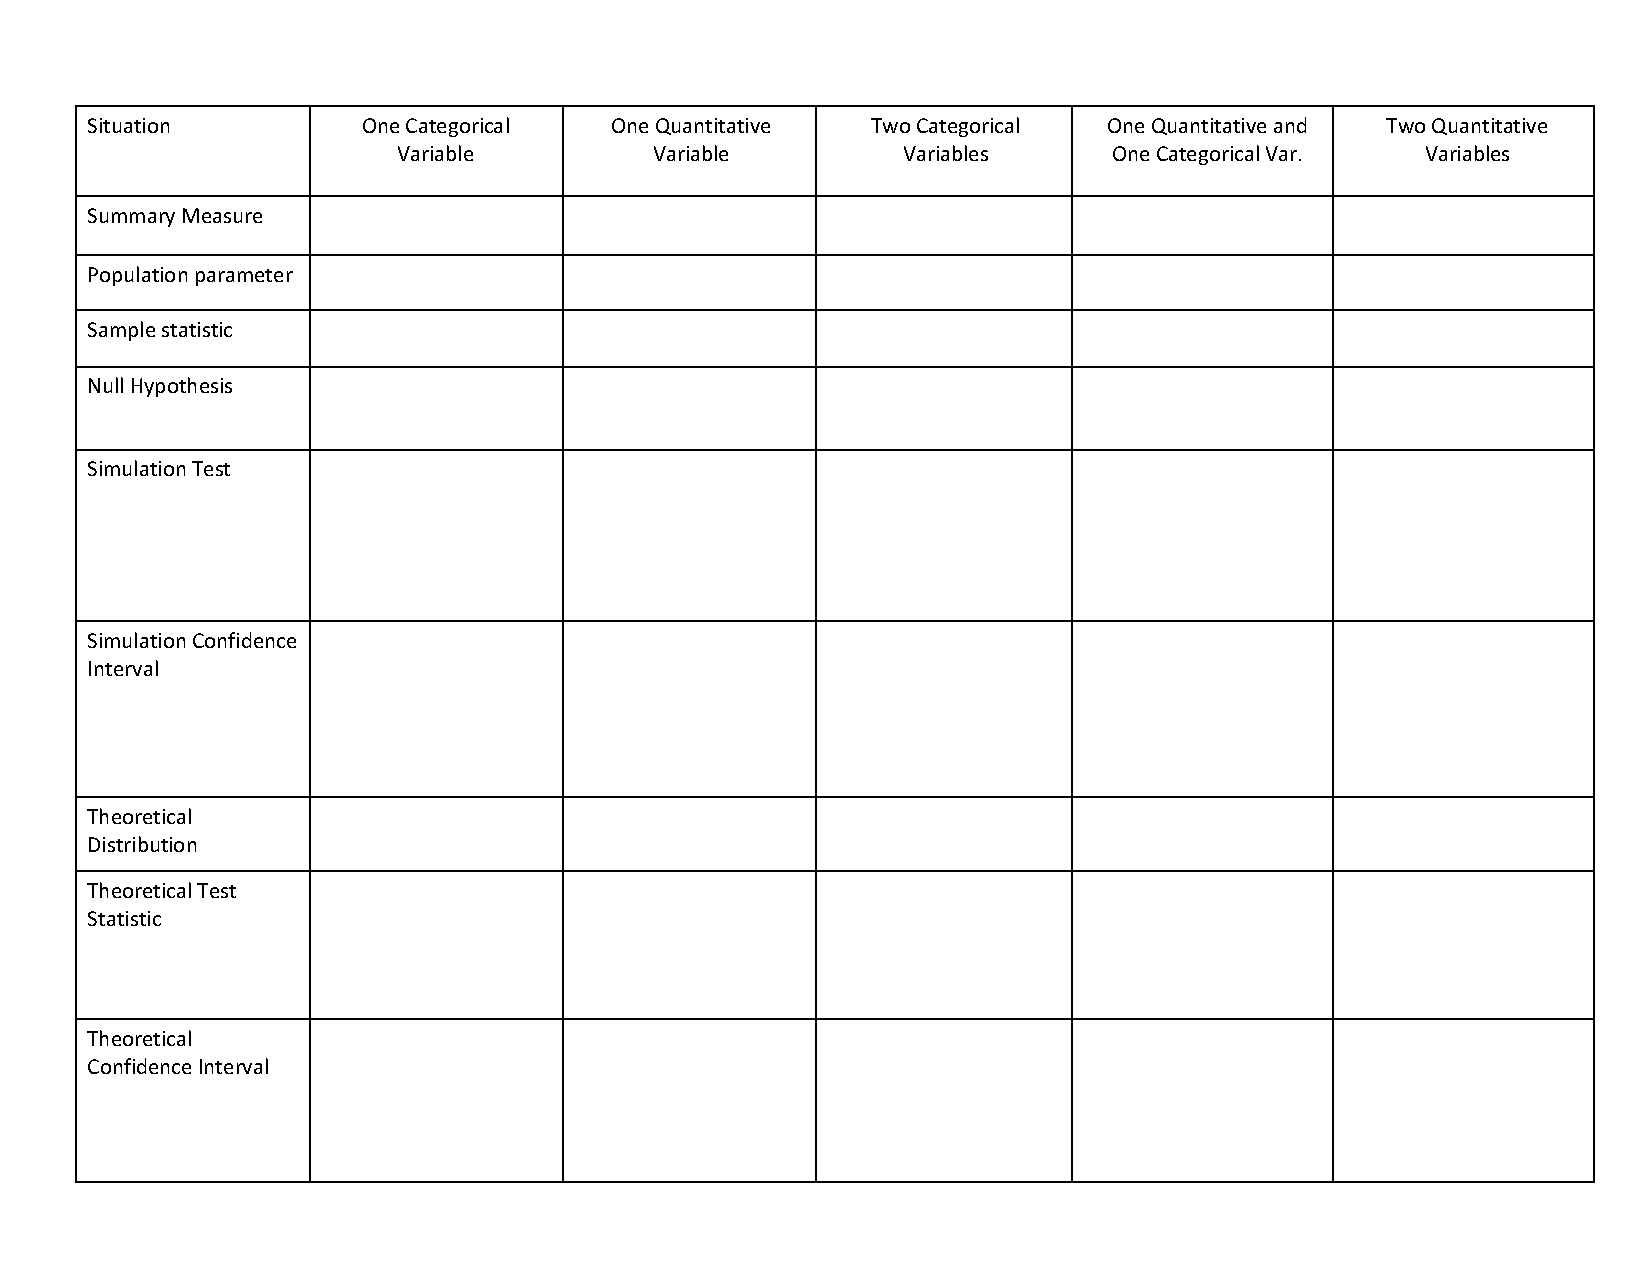
\includegraphics[angle = 90]{plots/ReviewTable.pdf}  %% p 253
    }
\end{figure}
\thispagestyle{empty}